% Lindenbaum algorythm
% - nodes with styles, 
% - turning lines without specifyng the corners

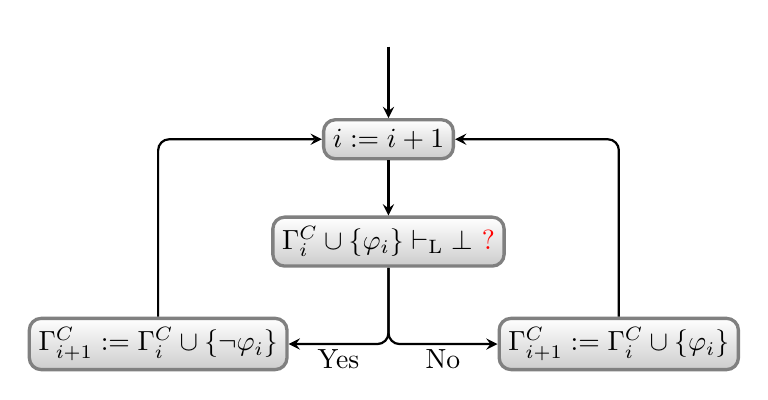
\begin{tikzpicture}[scale=1.3,>=stealth,
allapot/.style={ rectangle,minimum size=3mm,rounded corners=1.5mm,very thick,draw=black!50,top color=white,bottom color=black!20,
}]
\node(0) at (0,1){};
\node[allapot](i) at (0,0){$i:=i+1$};

\node[allapot](test) at (0,-1){$\Gamma_i^C \cup \{\varphi_i\}\vdash_{\mathrm{L}}\bot$ \textcolor{red}{?}};

\node[allapot](yes-case) at (-2.25,-2){$\Gamma_{i+1}^C := \Gamma_i^C\cup \{\lnot \varphi_i\}$};
\node[allapot](no-case) at (2.25,-2){$\Gamma_{i+1}^C := \Gamma_i^C\cup \{ \varphi_i\}$};

\begin{scope}[->, thick, rounded corners=4pt]
\draw (0)--(i);
\draw (i)--(test);
\draw (test)|-(no-case) node[pos=.75, below, inner sep=.5mm]{No};
\draw (test)|-(yes-case)node[pos=.75, below, inner sep=.5mm]{Yes};
\draw (yes-case)|-(i);
\draw (no-case)|-(i);
\end{scope}
\end{tikzpicture}
